\documentclass[../main.tex]{subfiles}
\begin{document}
\chapter{Dynamic Programming}
\begin{figure}[h]
    \centering
    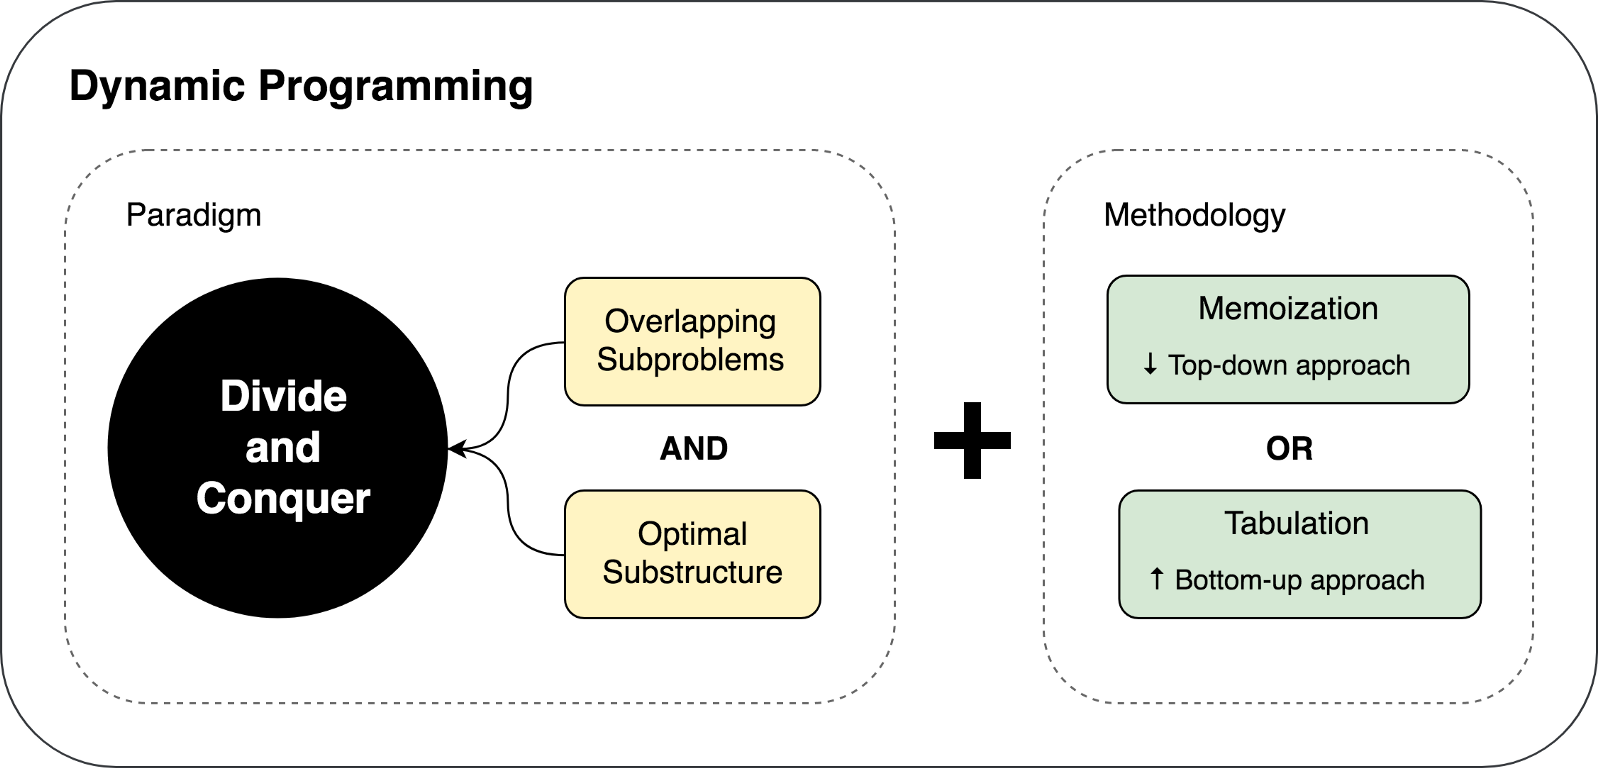
\includegraphics[width=0.95\columnwidth]{fig/dynamic_programming_chapter.png}
    \caption{Dynamic Programming Chapter Recap}
    \label{fig:dynamic_prorgramming_divide_conquer}
\end{figure}

% \begin{figure}[h!]
%     \centering
%     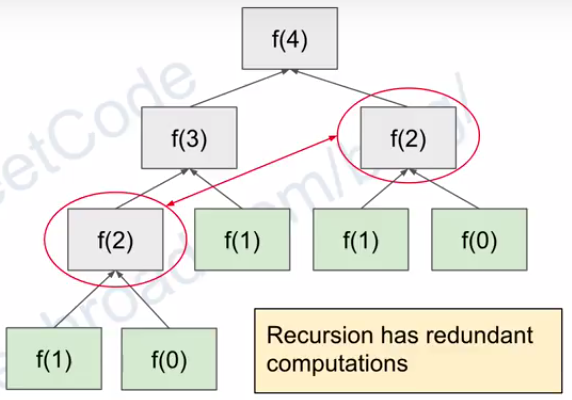
\includegraphics[width=0.7\columnwidth]{fig/fibanacci.png}
%     \caption{Fibonacci number's Recursion Tree}
%     \label{fig:fibonacci number}
% \end{figure}
% Use The subproblem graphs and  the recurrence function to denote the dynamic programming. 

Dynamic programming is simplifying a complicated problem by breaking it down into simpler sub-problems in a recursive manner. As introduced in Divide-and-Conquer in Chapter~\ref{chapter_divide_conquer}, dynamic programming is applied on problems wherein its subproblems overlap when you construct them in Divide-and-Conquer manner.  We use the recurrence function: $T(n) = T(n-1) + T(n-2) +...+T(1) + f(n)$, to highlight its most special characteristic -- Overlapping Subproblems -- compared with $T(n)=2T(n/2)+f(n)$ for Divide-and-Conquer's nonoverlapping subproblems.  As we shall see there are more types of recurrence functions in dynamic programming field other than this exemplary formulation, either in this chapter briefly or in Chapter~\ref{chapter_dynamic-programming} where a comprehensive list of dynamic programming categories/patterns are given.

\paragraph{Importance and Applications} Dynamic Programming is one of the fundamental methods in computer science and plays a very important role in computer algorithms, even the book \textit{artificial Intelligence, a modern approach} has mentioned this terminology for as many as 47 times. Dynamic programming firs for optimizing the problems fall into the following categories:
\begin{enumerate}
    \item Optimization: Compute the maximum or minimum value;
    \item Counting: Count the total number of solutions;
    \item Checking if a solution works.
\end{enumerate}
To be noticed, not that all problems with the above formats will be certainly solved with dynamic programing, it requires the problem to show two properties: overlapping subproblems and optimal substructures in order for dynamic programming to be applied. These two properties will be defined and explained in this chapter. 

\paragraph{Our Difference and Plan} A lot of textbooks or courses describe dynamic programming as obscure and demands creativity and subtle insights from users to identify and construct its dynamic programming solutions. However, we are determined to unfold such ``mystery'' by being grounding practical. We have two chapters topiced with dynamic programming: The current chapter oriented with clear definition by distinguishing, relating, and exampling the concept with divide-conquer and complete search. This chapter serves as the frontline of our contents on Dynamic Programming. Further, Chapter ~\ref{chapter_dynamic-programming} is focusing on categorizing problems patterns and giving examples on each. 

\begin{itemize}
    \item In order to understand how dynamic programming's role in the algorithms evolution map, the very first thing we do in Section~\ref{dynamic_programming_sec_search} is to show how we evolve the complete search to dynamic programming solution by: (1) discussing the relation between complete search, divide-and-conquer, and our dynamic programming; and (2) examining two elementary examples -- Fibonacci Sequence and Longest Increasing Subsequence. 
    \item Dynamic programming is typically applied on optimization problems. Section~\ref{sec_dynamic_programming_knowledge_base} discuss the principle properties, elements, and experience based guideline. And we show how we can relate these key characteristics to the field of optimization. 
    \item The naive solutions for dynamic programming applicable problems have either exponential or polynomial time using complete searching method. In Section.~\ref{sec_dynamic_programming_example} we showcase how we can decrease the complexity from the two baselines: from exponential to polynomial and  from polynomial to polynomial with lower power. 
\end{itemize}

% Follow the naive complete search, in this Chapter, we will first explain how to evolve the naive complete search solution to the dynamic programming using two examples: fibonacci sequence and longest increasing sequence in Section~\ref{dynamic_programming_sec_search}. Followed by this, we would have another second characterize the key elements of dynamic programming, and we give examples when dynamic programming used to optimize exponential or polynomial. In the second section, we give generalization: steps to solve the dynamic programming. and more related .






 %I explain the definition of dynamic programming, the three ways to implement it with Python, what types of dynamic programming we have, and how to solve each categories. 
% \paragraph{Dynamic Programming VS Divide and Conquer}
% For example, the famous fibonacci number $f(i) = f(i-2) + f(i-1)$ shown in Fig~\ref{fig:fibonacci number}. We divide the problem $i$ into two subproblems $i-2$ and $i-1$. If we want to obtain result for n, we would have n subproblems. This is different compared with our previous divide and conquer examples, which normally divide the problems into half and half. Because here each subproblem for example i, is one or two size larger than its previous subproblem.  Thus, the subproblems in dynamic programming \textit{overlapps} in some degree. Second, there is overlapping in dynamic programming's divided subproblems. We can find overlapping in two ways: 1) From the state transfer function; for example, $f(i-1) = f(i-3) + f(i-2)$, which means we computed $f(i-2)$ twice.  2) From the tree structure as shown in Fig~\ref{fig:fibonacci number}, where f(2) the subtree is computed twice. %This is the main difference between dynamic programming and Divide and conquer. 

\section{Introduction to Dynamic Programming}
\label{dynamic_programming_sec_search}
In this section, we answer two questions:
\begin{enumerate}
    \item \textbf{How to distinct divide and conquer from dynamic programming?} We have already conceptually know that it differs in the case of the characteristics of subproblems in two cases: overlapping subproblems for dynamic programming where each subproblems share subproblems and non-overlapping subproblems for divide and conquer where the subproblems are disjoint with each other. In this section, we further answer this question in a more visualized way using the concept of \textit{subproblem graph}. 
    \item \textbf{How to develop the dynamic programming solution from the complete search naive method? } We are not offering a fully and detail-oriented answer in this section. Instead, we first identify the problem using complete search in dynamic programming applicable problems using subproblem graph. Then we answer this question using two elementary examples by showing a sorted solutions so that we can demonstrate the relation between complete search and dynamic programming.
\end{enumerate}

\subsection{Concepts}
% Dynamic programming is an optimization methodology that used to improve efficiency from the problem's naive solution--complete search on subprogram graph (Depth-first-search and Breadth-first-search). 

\begin{figure}[ht!]
    \centering
    \begin{subfigure}[b]{0.3\textwidth}
    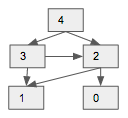
\includegraphics[width=\columnwidth]{fig/Subproblem_graph.png}
    \caption{Subproblem Graph for Fibononacci Sequence}
    \label{fig:subproblem_graph_1_fs}
    \end{subfigure}
    \begin{subfigure}[b]{0.65\textwidth}
    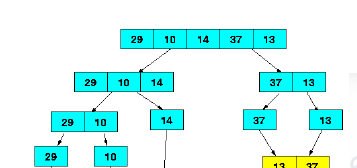
\includegraphics[width=\columnwidth]{fig/subproblem_graph_merge_sort.png}
    \caption{Subproblem Graph for Merge Sort}
    \label{fig:subproblem_graph_1_ms}
    \end{subfigure}
\caption{Subproblem Graph}
\label{fig:subproblem_graph_1}
\end{figure}

\paragraph{Subproblem Graph} If we treat each subproblem as a vertex, and the relation between subprblems as arced edges, we can get a directed subproblem graph. If the arced edge points from larger subproblems to smaller subproblems, we say it is in \textit{top-down fashion}. In contrast, if arced edge is pointing from smaller subproblems to large subproblems, it is \textit{bottom-up fashion}. In Fig.~\ref{fig:subproblem_graph_1} we draw the subproblem graph for Fibonacci Sequence which we have defined in Page\ref{} with $n=4$. In comparison, we also give the subproble m graph for sorting for array $[29, 10, 14, 37, 13]$. In the following contents, we show how we can use subproblem graph to answer the two questions we lay out at the beginning of this section. 
\paragraph{Terminologies} To make reading other materials accessible, we introduce more related terminologies that are widely used in the field.
\begin{itemize}
    \item \textbf{State}: State and subproblem is interchangeable among different books. Both of them can be used to describe the optimal solution to a problem with a solution space/search space. 
    \item \textbf{State Transition}: State transition and recurrence function is interchangeable. In the case of fibonacci sequence, our state transition/recurrence function is given as $f(n)=f(n-1)+f(n-2)$.  On the flip side, there are problems that will not specify the state transitions. We will have to figure them out by ourselves.
\end{itemize}

\paragraph{Distinction between Divide and Conquer and Dynamic Programming} In divide and conquer, problems are divided into disjoint subproblems, the subproblem graph would degrade to a \textit{tree structure}, each subproblem other than the base problems (here it is each individual element in the array) will only have out degree equals to 1. In comparison, in the case of fibonacci sequence shown in Fig.~\ref{fig:subproblem_graph_1}), some problems would have out degree larger than one, which makes the network a graph instead of a tree structure. This characteristics is directly induced by the fact that the subproblems overlap -- that is, subproblems share subprolems. For example, $f(4)$ and $f(3)$ share $f(2)$, and $f(3)$ and $f(2)$ shares $f(1)$. 

\paragraph{Complete Search and Dynamic Programming} If we program these two problems in a recursive top-down  divide-and-conquer manner, they are essentially equivalent to applying Depth-first-search on the subproblem graph/tree. The only difference is for sorting, there will be no recomputation (such as in merge sort and quick sort), while for the fibonacci sequence, subproblems that have in-degree larger than 1 will be recomputed multiple times, which gives us space for optimization and this is where the dynamic programming comes into rescue.  

With the subproblem graph, we reconstruct the problem as a graph problem, which means all complete searching methods can be applied; such as Breadth-first search other than the recursive depth-first-search. 

\paragraph{Depth-first-search} Because of the usage of subproblems, the depth-first-search implemented with divide-and-conquer manner (with the result of subproblems as return) outweight the usage of Breath-first-search. BFS doesn’t compute the values of “optimal” sub-solutions (of sub-instances) and use these to build up a solution, then build the optimum using this information. I don’t see anything “bottom-up” in the process of BFS. I don’t see where the “intermediate” states come. Therefore, we shall see that the close bond of dynamic programming with DFS instead of with BFS.

% We can also do a Breadth-first-search on the subproblem graph as an alternative choice. To draw the conclusion: \textit{complete search} on the subproblem graph is the most naive way to solve the dynamic programming possible problems. 

% \paragraph{Complete Search as Naive Solution}
% In Fig.~\ref{fig:subproblem_graph_1} shows the corresponding subproblem graph for Fibonacci sequence. We can see for some subproblems, e.g. node 2 and node 1 are both searched twice. Therefore, using the naive complete search method can led to redundant computation. 

\subsection{From Complete Search to Dynamic Programming}
\label{subsec_cs_to_dp}
So far, we know dynamic programming is an optimization methodology over the compete search solutions for typical optimization problems. Dynamic Programming's core principle is to solve each subproblem only \textit{once} by \textit{saving} and \textit{reusing} its solution. Therefore, compare with its naive counterpart -- Complete Search:
\begin{enumerate}
\item Dynamic Programming avoids the redundant recomputation met in its compete search counterpart as demonstrated in the last section.
    \item Dynamic Programming uses additional memory as a trade-off for better computation/time efficiency; it serves as an example of a \textit{time-space trade-off}. In most cases as we shall see in this chapter, the space overhead is well-worthy; it can decrease the time complexity dramatically from exponential to polynomial level.
\end{enumerate}

\paragraph{Two Forms of Dynamic Programming Solution}
There are two ways -- either recursive or iterative in general to add \textit{space mechanism} into naive complete search  to construct our dynamic programming solution. But do remember that we cannot eliminate recursive thinking completely. we will always have to define a recursive relation irrespective of the approach we use.
\begin{enumerate}
    \item \textbf{Top-down + Memoization (recursive DFS):} we start from larger problem (from top) and recursively search the subproblems space (to bottom) until the leaf node. This method is built on top of Depth-First Graph Search together with Divide and Conquer Methodology which treat each node as a subproblem and return its solution to its caller so that it can be used to build up its solution. Following a top-down fashion as is in divide and conquer, along the process, in the recursive call procedure, a hashmap is relied on to save and search solutions. The memoization works in such way that at the very first time that the subproblem is solved it will be saved in the hashmap, and whenever this problem is met again, it finds the solution and returns it directly instead of computing again. The key elements of this style of dynamic programming is:
    \begin{enumerate}
        \item Define subproblem;
        \item Develop solution using Depth-first Graph search and Divide and conquer (leave alone the recomputation).
        \item Adding hashmap to save and search the state of each subproblem.
    \end{enumerate}% In order to avoid the recomputation, we use a hashmap to save the solution to the solved subproblems, and whenever the subproblem is solved, we get its result from the hashmap instead of recompute its solution again. This method follows a top-down fashion. 
    \item \textbf{Bottom-up + Tabulation (iterative):} different from the last method,  which use recursive calls, in this method, we approach the subproblems from the smallest subproblems, and construct the solutions to larger subproblems using the tabulaized result. The nodes in the subproblem graph is visited in a \textit{reversed topological sort order}. This means that to reconstruct the state of current subproblem, all dependable (predecessors) have already be computed and saved. 
\end{enumerate}

\paragraph{Comparison}
The Figure~\ref{fig:dynamic_prorgramming_divide_conquer} record the two different methods, we can use \textit{memoization} and \textit{tabulation} for short.  Momoization and tabulation yield the same asymptotic time complexity, however the tabulation approach often has much better constant factors, since it has less overhead for procedure calls. 

The memoization method applies better for beginners that who have decent understanding of divide and conquer. However, once you study further and have enough practice, the tabulation should be more intuitive compared with recursive solution. Usually, dynamic programming solution to a problem refers to the solution with tabulation. 



We enumerate two examples: Fibonacci Sequence (Subsection~\ref{subsec_fibonacci_sequence}) and Longest Increasing Subsequence (subsection~\ref{subsec_longest_increasing_subsequence}) in the remaining section to showcase \textit{memoization} and \textit{tabulation} in practice. 

\subsection{Fibonacci Sequence}
\label{subsec_fibonacci_sequence}
\paragraph{Problem Definition}
% \begin{lstlisting}[numbers=none]
Given $f(0)=0, f(1)= 1, f(n) = f(n-1) + f(n-2), n>=2$. Return the value for any given $n$.
% \end{lstlisting}

As the most elementary and classical example demonstrating dynamic programming, we carry on this tradition and give multi-fold of solutions for fibonacci sequence. Since in Chapter.~\ref{chapter_divide_conquer} the recursive and naive solution is already given, we will just briefly explain it here. 

\paragraph{Complete Search}  Because the relation between current state and previous states are directly given, it is straightforward to solve the problem in a top-down fashion using depth-first search. The time complexity can be easily obtained from using induction or recurion tree: $O(2^n)$, where the base $2$ is the width of the tree, and $n$ is the depth. The Python code is given:
\begin{lstlisting}[language = Python]
# DFS on subproblem graph
def fibonacciDFS(n):
    # base case
    if n <= 1: return n
    return fibonacciDFS(n-1)+fibonacciDFS(n-2) # use the result of subtree to build up the result of current tree. 
\end{lstlisting}

\paragraph{Memoization} As we explained, there are subproblems computed more than once in the complete search solution. To avoid the recomputation, we can use a hashtable \texttt{memo} to save the solved subproblem. We need to make \texttt{memo} globally and available for all recursive calls; in the memoized complete search, instead of calling the recursion function $f(n) = f(n-1) + f(n-2)$ to get answer for current state $n$, it first check if the problem is already solved and available in \texttt{memo}. 

Because to solve f(n), there will be n subproblems, and each subproblem only depends on two smaller problems,  so the time complexity will be lowered to $O(n)$ if we use DFS+memoizataion. 
\begin{lstlisting}[language=Python]
# DFS on subproblem graph + Memoization
def fibonacciDFSMemo(n, memo):
    if n <= 1: return n
    if n not in memo:
        memo[n]= fibonacciDFSMemo(n-1, memo)+fibonacciDFSMemo(n-2, memo)
    return memo[n]
\end{lstlisting}

\paragraph{Bottom-up Tabulation} In the top-down recursive solution,  where exists two passes: one pass to divide the problems into subproblems, and the other recursive pass to gather solution from the base case and construct solution for larger problems. However, in the bottom-up tabulation way, for this specific problem, we have four key steps:
\begin{enumerate}
    \item We start by \textit{assigning} \texttt{dp} array to save each state's result.  It represents the fibonacci number at each  index (from 0 to $n$), which is also called a \textit{state}. 
    \item Then, we \textit{initialize} results of base cases which either were given or can be obtained easily with simple deduction. 
    \item We iterate through each subproblem/state in reversed topological sort order, which is $[0, 1, 2, 3, 4]$ as in Fig~\ref{fig:subproblem_graph_1}, and use tabulazied solution to build up the answer of current state through the given \textit{recurrence function} $f(n) = f(n-1) + f(n-2)$.  
    \item We return the last state in \texttt{dp} as the final \textit{answer}.
\end{enumerate}
The tabulation code of dynamic programming is given:
\begin{lstlisting}[language=Python]
# Dynamic Programming: bottom-up tabulation O(n), O(n)
def fibonacciDP(n):
    dp = [0]*(n+1)
    # init
    dp[1] = 1
    for i in range(2,n+1):
        dp[i] = dp[i-1] + dp[i-2]
    return dp[n]
\end{lstlisting}

% \textbf{BFS}. Here, I want to mention the BFS, because it can still solve dynamic programming related problems, sometimes in the shortest path problems can be especially helpful. Also, for BFS, it works better if accumulate result from root to the leaves, while in DFS, the result is brought back from leaves to the root. Also because BFS is naturally implemented iteratively without recursion and easier to understand compared with DFS, this is one advantage compared with DFS. The fibonacci number, however, it is difficult and inefficient to be solved using BFS. The tree structure is in Fig~\ref{fig:fibo_bfs}.  
% \begin{figure}[h]
%     \centering
%     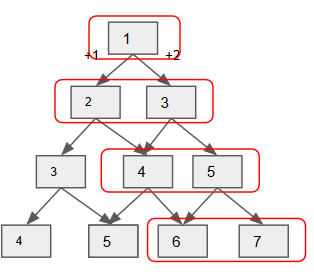
\includegraphics[width=0.6\columnwidth]{fig/fibonacci_bfs.png}
%     \caption{The BFS Tree structure for fibonacci sequence}
%     \label{fig:fibo_bfs}
% \end{figure}
% If we carefully design the queue of the BFS, which would only add the last two nodes. Then, the dp is filled in without repetition. And it is almost as efficient as the dynamic programming solution. 
% \begin{lstlisting}[language = Python]
% #Optimized BFS
% def FinonacciBFS(n):
%     dp = [0]*(n+1)
%     dp[1] = 1
%     bfs = [1]
%     dirs = [1, 2]
%     ans = 0
%     while bfs:
%         new_bfs = []
%         for i, v in enumerate(bfs):
%             for di in dirs:
%                 ni = v+di
%                 if ni<= n:
%                     dp[ni] += dp[v]
%                     if i == len(bfs)-1: #the last element
%                         new_bfs += [ni] 
%         bfs = new_bfs
%     return dp
    
% print(FinonacciBFS(9))
% # output
% # [0, 1, 1, 2, 3, 5, 8, 13, 21, 34]
% \end{lstlisting}
% \begin{lstlisting}[language = Python]
% # BFS
% def FinonacciBFS(n):
%     dp = [0]*(n+1)
%     dp[1] = 1
%     bfs = set([1]) #starts from 1 as root
%     dirs = [1, 2] #each move to 1 or 2.
%     ans = 0
%     while bfs:
%         new_bfs = set()
%         new_dp = [0]*(n+1)
%         for i in bfs:
%             for di in dirs:
%                 ni = i+di
%                 if ni<= n:
%                     new_dp[ni] += dp[i]
%                     new_bfs.add(ni)
%         bfs = new_bfs
%         dp = new_dp
%         ans += dp[n]
        
%     return ans
    
% print(FinonacciBFS(8))
% # output
% # 21
% \end{lstlisting}



% Thus, to get the dynamic programming solution, we need to figure out a way that we will fill out the results for all the states and each state will only dependent on the previous computed states.
% \subsection{Summary}
% For dynamic
%%%%%%%%%%%%%%Dynamic Programming Knowledge Base%%%%%%%%%%%%%%%%%%%%%%%%%%%%%%%%%
\section{Dynamic Programming Knowledge Base}
\label{sec_dynamic_programming_knowledge_base}
So far, we have learned most of the knowledge related to Dynamic programming, including basic concepts and two examples. In this section, we would officially answer three questions -- \textit{when} and \textit{how} to apply dynamic programming? and \textit{which} type of dynamic programming we need? Tabulation or Memoization. With clear definition, and offering some more practical guideline, complexity analysis, and comprehensive comprension between memoization and tabulation, we are determined to demystify dynamic programming. The subsections are organized as:
\begin{enumerate}
    \item Two properties and Practical Guideline (Section~\ref{sec_dp_two_properties}) that an optimization problems must have in order to answer the \textit{when} question.
    \item Five key elements, General Steps to Sovle Dynamic Programming, and Complexity Analysis (Section~\ref{sec_dp_elements}) in implementing the dynamic programming solution and to answer the \textit{how} question.
    \item Tabulation VS Memoization (Section~\ref{subsec_dp_comparison}) to answer the \textit{which} question. 
\end{enumerate} 

\subsection{When? Two properties}
\label{sec_dp_two_properties}
In order for the dynamic programming to apply, these two properties: overlapping subproblems and optimal substructure must be found in our solving problems. From our illustrated examples, 1) the step of identifying overlapping shows the overlapping subproblem properties. 2) the recurrence function in fact  shows the optimal substructure.   To be official, these two essential properties states as: 
\paragraph{Overlapping Subproblems}
When a recursive algorithm revisits the same subproblem repeatedly, we say that the optimization problem has overlapping subproblems. This can be easily visualized in the top-down subproblem graph, where one state is reached by multiple other states.  This property demonstrates the recomputation overhead seen in the complete search solutions of our two examples. 

Overlapping Subproblems property helps us find space for optimization and lead us to its solution -- \textit{the caching mechanism} used in dynamic programming. In the flip side, when subproblems are disjoint such as seen in merge sort and binary search, dynamic programming would not be helping.  
\paragraph{Optimal Substructure}
A given problem has optimal substructure property if the optimal solution of the given problem can be obtained by using optimal solutions of its subproblems. Only if optimal substructure property applied we can find the \textit{recurrence relation function} which is a key step in implementation as we have seen from the above two examples. Optimal substructures varies across problem domains in two ways:
\begin{enumerate}
    \item \textbf{Subproblem space:} how many subproblems an optimal solution to the original problem uses. For example, in Fibonacci sequence, each integer in range $[0, n]$ is a subproblem, which makes the $n+1$ as the total subproblem space. The state of each subproblem is the optimal solution for that subproblem which is $f(n)$. And in the example of LIS, each subproblem is the array with index in range $[0, i]$, and its state is the length of the longest increasing subsuquence ends/includes at index $i$, this makes the whole subproblem space to be $n$ too. 
    \item \textbf{State Choice:} how many choices we have in determining which subproblem(s) to use to decide the recurrence function for the current state. In Fibonacci sequence, each state only relies on two preceding states as seen in recurrence function $f(i)=f(i-1)+f(i-2)$, thus making it constant cost. For LIS, each state require knowing all inclusive states (solutions  relating to all smaller subproblems), which makes it cost of $O(n)$ that relates to the subproblem space. 
\end{enumerate}

Subproblem space and state choice together not only formulates the recurrent relation with which we very much have the implementation in hand. Together they also decide the time and space complexity we will need to tackle our dynamic programming problems. 

\paragraph{Practical Guideline}
Instead of the textbook definition, we also summarize the experience shared by experienced software programmers. Dynamic programming problems are normally asked in its certain way and its naive solution shows certain time complexity. Here, we summarize the situations when to use or not to use dynamic programming as \textbf{Dos} and \textbf{Donots}. 
\begin{itemize}
    \item  \textbf{Dos:} Dynamic programming fits for the optimizing the following problems which are either exponential or polynomial complexity using complete search:
\begin{enumerate}
    \item Optimization: Compute the maximum or minimum value;
    \item Counting: Count the total number of solutions; 
    \item Checking if a solution works.
\end{enumerate}

\item \textbf{Donots:}  In the following cases we might not be able to apply Dynamic Programming:
\begin{enumerate}
    \item When the naive solution has a low time complexity already such as $O(n^2)$ or $O(n^3)$.
    \item   When the input dataset is a set while not an array or string or matrix, $90\%$ chance we will not use DP.
    \item  When the overlapping subproblems apply but it is not optimization problems thus we can not identify the suboptimial substructure property and thus find its recurrence function. For example, same problem context as in \textbf{Dos} but instead we are required to obtain or print all solutions, this is when we need to retreat back to the use of DFS+memo(top-down) instead of DP. %, Draw out the tree structure is necessary and can be extremely helpful;

    %\item Get the total number of solutions. %(Need Correction}
\end{enumerate}
\end{itemize}
%%%%%%%%%%%%%%%%%%%%%%%%Four elements%%%%%%%%%%%%%%%%%%%%%%%%%%%%%%%
\subsection{How? Five Elements and Steps}
\label{sec_dp_elements}
In Section, we have provided two forms of dynamic programming solutions: memoization and tabulation, as two different ways of bringing the caching mechanism into practice. In this section, we focus on the iterative tabulation and generalize its four key elements and practical guidelines for import steps.

\paragraph{Five Key Elements of Tabulation}
As the first guideline of Tabulation, we summarize the four key elements  for the implementation of dynamic programming:
\begin{enumerate}
    \item \textbf{Subproblem and State:} Define what the subproblem space, what is the optimal state/solution for each subproblem. In practice, it would normally be the  \textit{the total/the maximum/minimum} for subproblem.  This requires us to know how to divide problem into subproblems, there are patterns to follow which will be detailed in Chapter.~\ref{}. 
    \item \textbf{State Transfer (Recurrence) Function}: derive the function that how we can get current state by using result from previous computed state(s). This requires us to identify the optimal substructure and  know how to make state choice.
    \item \textbf{Assignment and Initialization:} Followed by knowing the subproblem space, we typically assign a space data structure and initialize its values. For base or edge cases, we might need to initialize different than the other more general cases. 
    \item \textbf{Iteration:} decide the order of iterating through the subproblem space thus we can scan each subproblem/state exact and only \textit{once}. Using the subproblem graph, and visit the subproblms in reversed topological order is a good way to go.
    \item \textbf{Answer:} decide which state or a combination of all states such as the  the max/min of all the state is the final result needed. 
\end{enumerate}


%%%%%%%%%%%%%%Dynamic programming Dos and Do nots}
% \paragraph{Practical Guideline}
% \label{sec_dp_do_donots}
% From the above two examples in the last section, we can see that Dynamic programming can be potentialy used to optimize a exponential problem to be polynomial when it comes to problems asking for optimization, total number of solutions or if a resolution is working. For a problem that is already polynomial, dynamic programming can be potentially used to lower the complexity to BCR $O(n)$ just as shown in the second example. However, in this case the dynamic programming can be translated to other simple and straightforward  algorithm. To make the readers' life easier, in this book, we generalize the dos and do nots of dynamic programming so that you can have slightly more ideas about when to use dynamic prgramming and when to just use simpler algorithms for certain questions. 


\paragraph{Five Steps to Solve Dynamic Programming} This is a general guideline for dynamic programming -- memoization or tabulation. Key advice -- being ``flexbile''.  Given a real problem, all in all, we are credited with our understanding of the concepts in computer science. Thus, we should not be too bothered or stressed that if you can not come up with a ``perfect'' answer.  
\label{sec_dp_generalization}
\begin{enumerate}
    \item Read the question: search for the key words of the problem patterns: counting, checking, or maximum/minimum.
    \item Come up with the most naive solution ASAP:  analyze its time complexity. Is it a typical DFS solution? Try draw a SUBPROBLEM GRAPH to get visualization. Is there space for optimization?
    \item Apply Section~\ref{sec_dp_two_properties}: Is there overlapping? Can you define the optimal substructure/recurrence function?
    \item If the conclusion is YES, try to define the Five key elements so that we can solve it using the preferable tabulation. If you can figure it out intuitively just like that, great! What to do if not? Maybe retreat to use memoization, which is a combination of divide and conquer,  DFS, and memoization. 
    \item What if we were just so nervous that or time is short, we just go ahead and implement the complete search solution instead. With implementation is better than nothing. With the implementation in hand, maybe we can figure it out later. 
\end{enumerate}

\paragraph{Complexity Analysis}
\label{sec_dp_complexity_analysis}
The complexity analysis of the tabulation is seemingly more straightforward compared with its counterpart -- the recursive memoization. For the tabulation, we can simply draw conclusion without any prior knowledge of the dynamic programming by observing the \texttt{for} loops and its recurrence function. However, for both variant, there exists a common analysis method. The core points to analyze complexity involving dynamic programming is: (1) the subproblem space $|S|$, that is the total number of subproblems; and (2) the number of state choice needed to construct each state $|C|$. By multiplying these two points, we can draw the conclusion of its time complexity as $O(|S||C|)$.

For example, if the subproblem space is $n$ and if each state $i$ relies on (1) only one or two previous states as we have seen in the example of Fibonacci Sequence, it makes the time complexity $O(n)$; and (2) all previous states in range $[0, i-1]$ as seen in the example of Longest Increasing Subsequence, which can be viewed as $O(n)$ to solve each subproblem, this brings up the complexity up to $O(n^2)$.


\subsection{Which? Tabulation or Memoization}
\label{subsec_dp_comparison}
% \paragraph{Complete Search Assist to Dynamic Programming} Also, complete search can be used for us to further validate the solution or even help us to find the recurrence relation between subproblems in some cases. 
As we can see, the way the bottom-up DP table is filled is not as intuitive as the top-down DP as it requires some ‘reversals’ of the signs in Complete Search recurrence that we have developed in previous sections. However, we are aware that some programmers actually feel that the bottom-up
version is more intuitive. The decision on using which DP style is in your hand. To help you decide
which style that you should take when presented with a DP solution, we present the trade-off
comparison between top-down Memoization and bottom-up Tabulation in Table ~\ref{tab:dp_decidion_table}. 
\begin{table}[!ht]
\begin{small}
\centering
\noindent\captionof{table}{Tabulation VS Memoization}
\label{tab:dp_decidion_table}
 \noindent \begin{tabular}{|p{0.1\columnwidth}|p{0.43\columnwidth}|p{0.43\columnwidth}| }
  \hline
& Memoization& Tabulation   \\ \hline
Pros  &\begin{enumerate}[wide, labelwidth=!, labelindent=0pt,noitemsep,topsep=0pt]\item A natural transformation from normal recursive complete search.
    \item Compute subproblems only when necessary, sometimes this can be faster. 
\end{enumerate} &\begin{enumerate}[wide, labelwidth=!, labelindent=0pt,noitemsep,topsep=0pt] \item Faster if many sub-problems are revisited a sthere is no overhead of recursive calls.\item Can save memory space with dynamic programming `on-the-fly` technique (see Section Extension.~\ref{}). \end{enumerate}\\\hline
% \\ \hline
%  &\\ \hline
 Cons  & \begin{enumerate}[wide, labelwidth=!, labelindent=0pt,noitemsep,topsep=0pt]
     \item Slower if many subproblemes are revisited due to overhead of recursive calls. 
     \item If there are $n$ states, it can use up to $O(n)$ table size which might lead to Memory Limit Exceeded(MLE) for some hard problems. 
     \item Faces stack overflow due to the resursive calls.
 \end{enumerate} &
 \begin{enumerate}[wide, labelwidth=!, labelindent=0pt,noitemsep,topsep=0pt]
     \item For programmers who are inclined with recursion, this may not be intuitive.
    %  \item If there are $n$ states
 \end{enumerate}\\ \hline
\end{tabular}
\end{small}
\end{table}


%%%%%%%%%%%%%%%%%%%%%%%%%%%%%%%%%%%%%%%%%%%%%%%%%%%%%%%%%%%%%%%%%%%%%%%%%%%%%%%%%%%%%%%%%%%%%%%%%%
%%%%%%%%%%One Dimensional State VS Multiple Dimensional State%%%%%%%%%%
%%%%%%%%%%%%%%%%%%%%%%%%%%%%%%%%%%%%%%%%%%%%%%%%%%%%%%%%%%%%%%%%%%%%%%%%%%%%%%%%%%%%%%%%%%%%%%%%%%%
\section{Hands-on Examples (Main-course Examples)}
\label{sec_dynamic_programming_example}

In the practical guideline, we mentioned that the problems that can be further optimized with dynamic programming would be seen with  complexity patters of their naive solutions: either exponential such as $O(2^n)$ or polynomial such as $O(n^3)$ or $O(n^2)$.

The purpose of this section is to further enhance our knowledge and put our both theoreotical and practical guideline into test.  We examine two examples: Triangle and maximum subarray. We have seen how maximum subarray can be solved with linear search and divide and conquer in Chapter.\ref{}. However, in this section, we expand the old solution into dynamic programming solutions and we see the difference and connection. %Dynamic programming can decrease the complexity that used divide and conquer or searching from exponential level to polynomial, e.g. from $O(2^n)$ or $O(n!)$ to $O(n^m)$, $m$ usually is $2$ or $3$. 

%Let us see two more examples: The first one is to optimize a $O(2^n)$ problem, the second one is to optimize a $O(n^3)$ problem.

\subsection{Exponential Problem: Triangle}
\paragraph{Triangle (L120)} 
Given a triangle, find the minimum path sum from top to bottom. Each step you may move to adjacent numbers on the row below.
\begin{lstlisting}[numbers=none]
Example:
Given the following triangle:

[
[2],
[3,4],
[6,5,7],
[4,1,8,3]
]
The minimum path sum from top to bottom is 11 (i.e., 2 + 3 + 5 + 1 = 11).
\end{lstlisting}

  
\paragraph{Analysis}
\begin{enumerate}
    \item We quickly read the question and we find the key word -- minimum.
    \item We come up with the most naive solution that would be dfs which we have already covered in chapter. A quick drawing of dfs traversal graph, we can find some nodes are repetitively visited. 
    \item Apply Two Properties: First, define the subproblem, for each node in the triangle, it is decided by two indexes $(i, j)$ as row and column index respectively. The subproblem can be straightforward, the minimum sum from the starting point $(0, 0)$ to current position $(i, j)$. And the subprogram graph will be exactly the same as the graph we used in dfs. We identify overlapping easily. 
    
    Now, develop the recurrence function. To build up solution for state at $(i, j)$, it needs two other states: $(i-1, j)$ and $(i-1, j-1)$ and need one value from current state. The function will be: $f(i, j)=\min(f(i-1, j), f(i-1, j-1)) + t[i][j]$.
    \item Five Key Elements: we need to figure out how to assign and initialize the \texttt{dp} space and do the iteration. To get the boundary condition:
    \begin{enumerate}
        \item by observation: the first element at $(0, 0)$ will have none of these two states $f(i-1, j), f(i-1, j-1)$ exist. the leftmost and rightmost element of the triangle will have only one of these two states: $f(i-1, j), f(i-1, j-1)$. 
        \item by simple math induction: $i \in [0, n-1], j \in [0, i]$. When $i=0, j=0$, $f(i, j)=t[i][j]$, when $i \in [1, n-1], j=0$, $f(i-1, j-1)$ is invalid, and when $i=n-1, j=n-1$, $(i-1, j)$ is invalid.
    \end{enumerate}
    The answer would be the minimum value of \texttt{dp} at the last row.
    The Python code is given:
    
    \begin{lstlisting}[language = Python]
def min_path_sum(t):
    dp = [[0 for c in range(r+1)] for r in range(len(triangle))] # initialized to 0 for f()
    n = len(triangle)
    #initialize the first point, bottom
    dp[0][0] = triangle[0][0]
    #initial the left col and the right col of the triangle
    for i in range(1, n):
        dp[i][0] = dp[i-1][0] + dp[i][0]
        dp[i][i] = dp[i-1][i-1] + dp[i][i]
    for i in range(1, n):
        for j in range(1, i):
            dp[i][j] = t[i][j] + min(dp[i-1][j], dp[i-1][j-1])
    return min(dp[-1])
\end{lstlisting}
\end{enumerate}
% In section of graph search, we have seen the dfs solution of triangle. If 
% In the above solution, the state is a recursive tree, and the DFS traverse all the elements in the tree. To reformulate this problem as dynamic programming, if we use $f[x][y]$ marks the minimum path sum start from $(x,y)$, then we have this relation $f[x][y] = A[x][y] + min(f[x+1][y], f[x+1][y+1]$, which gives us a function $T(n) = 2*T(n-1)$. We still have $O(2^n)$ time complexity and still encounter LTE error. 
% \begin{lstlisting}[language = Python]
% def minimumTotal(triangle):
%     def divideConquer(x, y):
%         if x == len(triangle):
%             return 0
%         return triangle[x][y]+min(divideConquer(x+1, y), divideConquer(x+1, y+1))
%     return divideConquer(0, 0)
% \end{lstlisting}
% \textbf{Recursive and Memoization} 

% Here, for location $(x ,y)$ we need to compute $(x+1, y+1)$, for location $(x , y+1)$, $f[x][y+1] = A[x][y+1] + min(f[x+1][y+1], f[x+1][y+2]$, we compute $(x+1, y+1)$ again. So the redundancy exists. However, the advantage of this formate with divide and conquer compared with DFS brute force is that we can use memoization to trade for speed and save complexity. Till now the code is successfully AC. 

% The time complexity here is propotional to the number of subproblems, which is the size of triangle, $O(n^2)$. This is usually not obvious of its complexity. 
% \begin{lstlisting}[language = Python]
% from sys import maxsize
% def minimumTotal(triangle):
%     memo = [[maxsize for i in range(j+1)] for j in range(len(triangle))]
%     def divideConquerMemo(x, y):
%         #nonlocal memo
%         if x == len(triangle):
%             return 0
%         if memo[x][y] == maxsize:
%             memo[x][y] = triangle[x][y] + min(divideConquerMemo(x+1, y), divideConquerMemo(x+1, y+1))
%         return memo[x][y]
%     return divideConquerMemo(0, 0)
% \end{lstlisting}
% It is normally 
% \textbf{Iterative with Space}
% Now, we do not use the recursive function, the same as the above memoization, we use a memo space f to save the result. This implementation is more difficult compared with the recursive + memoization method. But it is still something managable with practice. The advantages include:
% \begin{enumerate}
% \item It saves the heap space from the implementation of the recursive function. 
% \item It is easier to get the complexity of the algorithm compared with recursive implementation, simply by looking at its for loops. 
% \item It is easier to observe the value propagation order, which make it possible to optimize the space complexity.
% \end{enumerate}

% For the iterative, we have two ways: Bottom-up and top-down. This is compared with your order to fill in the dynamic table.   If we use our previous defined relation function $f[x][y] = A[x][y] + min(f[x+1][y], f[x+1][y+1]$,  we need to know the result from the larger index so that we can fill in value at the smaller index. Thus,  we need to initialize the result for the largest indices. And we reversely fill in the dynamic table, this is called top-down method, from big index to small. Visually we propagate the information from the end to the front. The final result

% On the other side, if we fill in the table from small to larger index, we need to rewrite the relation function to $f[x][y] = A[x][y] + min(f[x-1][y], f[x-1][y-1]$, this function feedforward the information from the beginning to the end. So we need to initialize the result at (0,0), and the edge of the triangle. following the increasing order, to get value for the larger index, it is bottom-up method. 




% \textbf{Top-down with standard space} $f[x][y] = A[x][y] + min(f[x+1][y], f[x+1][y+1]$. Actually for this problem, the top-down method is slightly simpler: we only need to initialize the last row for the state $f$ because for the last row, we cant find its previous state. We directly return result of $f[0][0]$.
% \begin{lstlisting}[language = Python]
% # top-bottom
% from sys import maxsize
% def minimumTotal(triangle):
%     f = [[0 for i in range(j+1)] for j in range(len(triangle))] # initialized to 0 for f()
%     n = len(triangle)
%     #initial the the last row
%     for y in range(len(triangle[-1])):
%         f[-1][y] = triangle[-1][y]
%     # from small index to large index
%     for x in range(n-2, -1, -1):
%         for y in range(x, -1, -1):
%             f[x][y] = triangle[x][y] + min(f[x+1][y], f[x+1][y+1]) #get result for larger state from smaller state
%     return f[0][0]
% \end{lstlisting}
\paragraph{Space Optimization} From the recurrence function, we can see the current state is only related to two states from the last row. We can reuse the original \texttt{triangle} matrix itself to save the state. If we are following the forward induction as the previous solution, we still have the problem of edge cases; for some state that it only has one previous or none previous states needed to decide its current state. We can write our code as: 
\begin{lstlisting}[language=Python]
def min_path_sum(t):
    '''
    Space optimization with forward induction
    '''
    t = deepcopy(t)
    if not t:
      return 0
    n = len(t)
    for i in range(0, n):
        for j in range(0, i + 1):
            if i == 0 and j == 0:
              continue
            elif j == 0:
              t[i][j] = t[i][j] + t[i-1][j]
            elif j == i:
              t[i][j] = t[i][j] + t[i-1][j-1]
            else:
              t[i][j] = t[i][j] + min(t[i-1][j], t[i-1][j-1])
    return min(t[-1])
\end{lstlisting}
\paragraph{Further Optimization} Let us look at the traversal order backward where we start from the last row and traverse upward to the first row. For the last row, its state should be the same as its triangle value. For any remaining rows and each of its element, its state will all rely on two other states locating below of them. There is consistency in this backward induction and the final state at the first row will be only final global answer.  In this method, we reverse of recurrence function as $f(i,j)=min(f(i+1, j+1), f(i+1, j))+t[i][j]$.
\begin{lstlisting}[language = Python]
def min_path_sum(t):
    '''
    Space optimization with backward induction
    '''
    t = deepcopy(t)
    if not t:
      return 0
    n = len(t)
    # Start from the last second row
    for i in range(n-2, -1, -1):
        for j in range(i, -1, -1):
            t[i][j] = t[i][j] + min(t[i+1][j], t[i+1][j+1])
    return t[0][0]
\end{lstlisting}

%%%%%%%%%%%%%%%%%%%%%%%%%%%%%%%%%%%%% materials needed 
%https://blog.csdn.net/github_30242787/article/details/50819414
%https://blog.csdn.net/xiaqian0917/article/details/53266662

\subsection{Polynomial Problem: Maximum Subarray}

\paragraph{Maximum Subarray (L53)} Find the contiguous subarray within an array (containing at least one number) which has the largest sum. 
\begin{lstlisting}[numbers=none]
For example, given the array [-2,1,-3,4,-1,2,1,-5,4], the contiguous subarray [4,-1,2,1] has the largest sum = 6.
\end{lstlisting}

The problem will be analyzed following our two properties and solved following our five step guideline and five elements. 
% \paragraph{Apply Five Steps} Let
\paragraph{Analysis and $O(n)$ Solution}

\begin{enumerate}
    \item First step, we read the problem and we can quickly catch the key word -- maximum.  

\item Second step, the naive solution. We have From other chapters, we have seen how maximum subarray can be approached as either graph search ($O(2^n)$ \textcolor{red}{to get more details later}), linear search along the solution space ($O(n^3)$ and $O(n^2)$ if be tweeted with the computation of subarray). 

\item Third step: Apply two properties. The solution space we concluded for maximum subarray would be totally in $O(n^2)$, and be denoted as $a[i, j]$ where $i, j \in [0, n-1], j \leq i$. This states that the maximum subarray is one of these subarrays fixing their starting index.  Here, in order to think in dynamic programming way, let us define subproblem. We first define it as $a[i, j]$, and the state would be its sum of this subarray. We can see there is already some hidden recurrence function that $f(i, j)=f(i,j-1)+a[j]$. We would see there is overlap: $a[0, 4]$ actually includes $a[1, 4]$. 

However, there is something missing. The state we define did not take leverage of the optimal substructure. Let us define the subproblem in another way that has the optimal condition there. We define $f(i), i \in [0, n-1]$, represents the  subarry that starts from index $i$ and the answer/state will be the maximum value of these potential subarrarys. Therefore, the subproblem space will be only $O(n)$. The solution space of subproblem $f(i)$ is $a[i, j]$ where $i, j \in [0, n-1], j \leq i$. Assume we are comparing $f(0)$ and $f(1)$, that is the relation of maximum subarry starts from 0 and the maximum subarry that starts from 1. $f(1)$ is a subproblem of $f(0)$. If $f(1)$ is computed already, the $f(0)$ would be either include $f(1)$ if its positive or not include with two possible state-choice. Thus, we get our recurrence function $f(i-1)=max(f(i)+a[i], a[i])$. The last state is $f(n-1)=a[n-1]$. 

\item Step 4: Given all the conclusions, we can start the five key elements. The above solution requires us to start from the maximum index in a reverse order, this is called \textit{backward induction} mentioned in materials explaining dynamic programming from the angle of optimization. We need to always pay attention there is empty array where the maximum subarray should give zero as result. This makes our total states $n+1$ instead of $n$. In the backward induction, this empty state will locate at index $n$ with a list of size $n+1$. %What we can do that is more intuitive is a forward deduction. 

\begin{lstlisting}[language = Python]
def maximum_subarray_dp(a):
  '''
  Backward induction dp solution
  '''
  # assignment and initialization
  dp = [0] * (len(a) + 1)
  # fill out the dp space in reverse order
  # we do not need to fill the base cae dp[n]
  for i in reversed(range(len(a))):
    dp[i] = max(dp[i+1] + a[i], a[i])
  print(dp)
  return max(dp)
\end{lstlisting}
\end{enumerate}


% Brute Force solution: put it into
% The brute force solution of this problem is to use two for loops, one pointer at the start position of the subarray, the other point at the end position of the subarray. Then we get the maximum sum of these subarries. The time complexity is $O(n^3)$, where we spent $O(n)$ to the sum of each subarray. However, if we can get the sum of each subarray with $O(1)$. Then we can lower the complexity to $O(n^2)$. Here one solution is to get $sum(i+1) = sum(i)+nums[i+1]$. 
% \begin{lstlisting}[language=Python]
% from sys import maxsize
% def maximumSubarray(nums):
%     if not nums:
%         return 0
%     maxValue = -maxsize
%     for i, v in enumerate(nums):
%         accSum = 0
%         for j in range(i, len(nums)):
%             #accSum = sum(nums[i:j+1])
%             accSum += nums[j]
%             maxValue = max(maxValue, accSum)
%     return maxValue
% \end{lstlisting}
% Another way that we can get the sum between $i,j$ in $O(1)$ time with formula $sum(i,j)=sum(0,j)-sum(0,i)$ by using $O(n)$ space to save the sum from $0$ to current index. %is to trade space for efficiency. the sum of subarray from index $i$ to $j$ is $sum(i,j)=sum(0,j)-sum(0,i)$. We can pre compute the accumulated sum to each index and save it in an array of the same size, which gives us $O(n^2)$ time complexity and $O(n)$ space complexity.  The code is writen as: 

% solution: Divide and Conquer
% To further improve the efficiency, we use divide and conquer, where we divide one array into two halves: the maximum subarray might located on the left size, or the right side, or some in the left side and some in the right size, which crossed the bound. $T(n) = max(T(left),T(right), T(cross))$, max is for merging and the T(cross) is for the case that the potential subarray across the mid point. For the complexity, $T(n)=2T(n/2)+n$, if we use the master method, it would give us $O(nlgn)$. With this solution, we use $O(lgn)$ space for the recursive function stack space.
% \begin{lstlisting}[language=Python]
% def maxSubArray(self, nums):
%         """
%         :type nums: List[int]
%         :rtype: int
%         """
%         def getCrossMax(low,mid,high):
%             left_sum,right_sum =0,0
%             left_max,  right_max = -maxint, -maxint
%             left_i,right_j=-1,-1
%             for i in xrange(mid,low-1,-1): #[)
%                 left_sum+=nums[i]
%                 if left_sum>left_max:
%                     left_max= left_sum
%                     left_i = i
%             for j in xrange(mid+1,high+1):
%                 right_sum+=nums[j]
%                 if right_sum>right_max:
%                     right_max= right_sum
%                     right_j = j
%             return (left_i,right_j,left_max+right_max)
        
%         def maxSubarray(low,high):
%             if low==high:
%                 return (low,high, nums[low])
%             mid = (low+high)//2
%             rslt=[]
%             #left_low, left_high, left_sum = maxSubarray(low,mid) #[low,mid]
%             rslt.append(maxSubarray(low,mid)) #[low,mid]
%             #right_low,right_high,right_sum = maxSubarray(mid+1,high)#[mid+1,high]
%             rslt.append(maxSubarray(mid+1,high))
%             #cross_low,cross_high,cross_sum = getCrossMax(low, mid, high)
%             rslt.append(getCrossMax(low, mid, high))
%             return max(rslt, key=lambda x: x[2])
%         return maxSubarray(0,len(nums)-1)[2]
% \end{lstlisting}

% Dynamic Programming: Using dynamic programming: the $f$ memorize the maximum subarray value till $j$, the state till $i$ we can get the result from previous state $i-1$, the value of current state depends on the larger one between $f[i-1]$ plus the current element and the current element, which is represented as $f[i] = max(f[i-1] + nums[i], nums[i])$. This would gave us $O(n)$ time complexity and $O(n+1)$ space complexity. The initialization is $f[0] = 0$, and the answer is $max(f)$.

\paragraph{Space Optimization}

If we observe the iterating process, we always only use one previous state. If we use another global variable, say \texttt{maxsum} to track the global maximum subarray value, and use \texttt{state} to replace \texttt{dp} array, we can decrease the space complexity from $O(n)$ to $O(1)$. %However, here since we only need to track $f[i]$ and $f[i+1]$, and keep current maximum value, so that we do not need to use any space. 
\begin{lstlisting}[language = Python]
def maximum_subarray_dp_sp(a):
  '''
  dp solution with space optimization
  '''
  # assignment and initialization
  state = 0
  maxsum = 0
  # fill out the dp space in reverse order
  # we do not need to fill the base cae dp[n]
  for i in reversed(range(len(a))):
    state = max(state + a[i], a[i])
    maxsum = max(maxsum, state)
  return maxsum
\end{lstlisting}

All of the above steps are for deep analysis purpose. When you are more experience, we can go directly to the five elements of tabulation and develop the solution without connecting it to the naive solution. Also, this is actually a Kadane's Algorithm which will be further detailed in Chapter.~\ref{}. 



% \subsection{Implementations}
% There are different ways to implement dynamic programming: 1) recursive$+$ memoization; including top-down and down-top. 2) iterative $+$ memozation; including top-down and down-top. Also, in a lot of scenarios, we can optimize the space complexity too. For example, rolling array. 
% \subsubsection{Recursive and Memoization}
% This method is the most direct and the easiest way to solve the problems. For example. However, this method because it uses recursive function, which include extra space compared with the following iterative method.
% \subsubsection{Iterative}
% We can avoid recursion by using multiple levels of for loop. The four key elements that to design an iterative dynamic programming are:

% \begin{enumerate}
%     \item State: how to represent the solution, maximum or minimum, Yes or No, count; 
%     \item Function: the state transfer between smaller state and larger state;  
%     \item Initialization: The smallest state, base state and its solution, which is the start; 
%     \item Answer: what is the largest state, which is the end.
% \end{enumerate}
% where we can get the result of a problem by iteratively "growing" from the smaller problems. To find the transfer function, the best way to do it is to get a example of each scenario, and see for each case, to decide the relation between smaller problems and larger problems. 

% % now give examples to this section
% \section{Derive Dynamic Programming from BFS}
% \begin{lstlisting}[language = Python]
% def uniquePaths(self, m, n):
%         """
%         :type m: int
%         :type n: int
%         :rtype: int
%         """
%         if m==0 or n==0:
%             return 0
%         d = [(1, 0), (0, 1)]
%         count =[[0 for col in range(n)] for row in range(m)]
%         count[0][0]=1
%         bfs = [(0,0)]
%         while bfs:
%             new_bfs = set()
%             for x, y in bfs:
%                 for dx, dy in d:
%                     posX, posY = x+dx, y+dy
%                     if 0<=posX<m and 0<=posY<n: #valid and not be visited before
%                         count[posX][posY] += count[x][y]
%                         new_bfs.add((posX, posY))
%             bfs = list(new_bfs)
%         return count[-1][-1]
% \end{lstlisting}




% \subsection{Single-Choice and Multiple-Choice State, put it into complexity}
% Generally speaking, given a sequence,  if the final solution can be constructed from a subproblem that choose a certain element from its current state, then it is a single state dynamic programming problem. For example, the Longest increasing subsequence problem. On the other hand, for the subproblem, we can have multiple choice, and the optimal solution can be dependenable on all of  these different states. For example, 801. Minimum Swaps To Make Sequences Increasing. Knowing how to solve problems that has multiple-choice state is necessary. 
% \subsubsection{Two-Choice State}






%%%%%%%%%%%%%%%%%%%%%%%%%%%%%%%%%%%%%%%%%%%%%%%%%%%%%%%%%%%%%%%%%%%%%%%%%%%%%%%%%%%%%%%%%%%%%%%%%%
%%%%%%%%%%Exercise%%%%%%%%%%
%%%%%%%%%%%%%%%%%%%%%%%%%%%%%%%%%%%%%%%%%%%%%%%%%%%%%%%%%%%%%%%%%%%%%%%%%%%%%%%%%%%%%%%%%%%%%%%%%%%
% \section{Time Complexity Analysis}
% \subsubsection{Substitution Method}
% The substitution method comprises two steps to solving the recurrence and the the either the upper bound or lower bound time complexity. 
% \begin{enumerate}
%     \item Guess the form of the solution.
%     \item Use mathematical induction to find the constants and show that the solution works.
% \end{enumerate}
% For example, given a recurrence equation as follows:
% \begin{equation} \label{eg_recurrence_1}
% \begin{split}
% T(n) & = 2T(\floor*{n/2}) + n\\
% \end{split}
% \end{equation}
% We guess the upper bound time complexity is $O(nlgn)$, which is to say we need to prove that $T(n)\leq cnlgn$ for an appropriate choice of the constant $c > 0$.  We start by assuming that this holds true for some smaller $m<n$, here we let $m = \floor*{n/2}$, which yields $T(\floor*{n/2})\leq c\floor*{n/2} lg(\floor*{n/2})$, then we substitute $T(\floor*{n/2})$ into Eq.~\ref{eg_recurrence_1}, we have the following inequation:
% \begin{equation} \label{eg_recurrence_2}
% \begin{split}
% T(n) &\leq 2 (c\floor*{n/2} lg(\floor*{n/2})) + n\\
% &\leq cnlg(n/2) +n\\
% &\leq cnlgn - cnlg2 + n \\
% &\leq cnlgn -cn + n\\
% &\leq cnlgn, \text{if} c\geq 1, 
% \end{split}
% \end{equation}

% Unfortunately, it could be difficult to come up with an asymptotic guess (that as close as the above one). It takes experience. Fortunately, we still have two ways that help us to make a better guess. 
% \begin{enumerate}
%     \item We can draw a recursive tree that visually helps us make a heuristic guess. 
%     \item We can make a guess to prove the loose upper and lower bounds on the recurrence and then reduce the range of uncertainty. 
% \end{enumerate}
% Also, for our guess, if we directly substitute we can not always prove the induction. Consider the recurrence:
% \begin{equation} \label{eg_recurrence_3}
% \begin{split}
% T(n) & = T(\floor*{n/2}) + T(\ceil*{n/2})+1, \\
% \end{split}
% \end{equation}
% A reasonable and logical guess for this recurrenc is $T(n) = O(n)$, so that we obtain
% \begin{equation} \label{eg_recurrence_4}
% \begin{split}
% T(n) & \leq c\floor*{n/2} + c (\ceil*{n/2})+1, \\
% & = cn+1
% \end{split}
% \end{equation}
% However, the induction is not exactly having $cn$ as an upper bound, but it is constant close enough. If we are just in the coding interview, we do not need to bother two much about slightly subtleties.
\section{Exercises}
\subsection{Knowledge Check}
\begin{enumerate}
    \item The completeness of Dynamic programming. 
\end{enumerate}
\subsection{Cooding Practice}
In order to understand how the efficiency is boosted from searching algorithms to dynamic programming, readers will be asked to give solutions for both searching algorithms and dynamic programming algorihtms. And then to compare and analyze the difference. (Two problems to be asked) 
\begin{enumerate}


\item \textbf{Coordinate Type} 63. Unique Paths II (medium).

A robot is located at the top-left corner of a m x n grid (marked 'Start' in the diagram below).

The robot can only move either down or right at any point in time. The robot is trying to reach the bottom-right corner of the grid (marked 'Finish' in the diagram below).

Now consider if some obstacles are added to the grids. How many unique paths would there be?

An obstacle and empty space is marked as 1 and 0 respectively in the grid.

Note: m and n will be at most 100.

Example 1:
\begin{lstlisting}
Input:
[
  [0,0,0],
  [0,1,0],
  [0,0,0]
]
Output: 2
\end{lstlisting}
Explanation:
There is one obstacle in the middle of the 3x3 grid above.
There are two ways to reach the bottom-right corner:
\begin{lstlisting}
1. Right -> Right -> Down -> Down
2. Down -> Down -> Right -> Right
\end{lstlisting}

\textbf{Sequence Type}

\item 213. House Robber II

Note: This is an extension of House Robber.

After robbing those houses on that street, the thief has found himself a new place for his thievery so that he will not get too much attention. This time, all houses at this place are arranged in a circle. That means the first house is the neighbor of the last one. Meanwhile, the security system for these houses remain the same as for those in the previous street.

Given a list of non-negative integers representing the amount of money of each house, determine the maximum amount of money you can rob tonight without alerting the police.

example
 nums = [3,6,4], return 6

% 现在呢, 我们如果选3了的话, 4不好搞。

% 如果选4了的话呢, 3不好搞。
%  这就变成了一个循环数组问题, 循环数组问题有三种方法可以解:

%     取反
%     分裂
%     倍增

% 这里我们用分裂的方法, 把数组

% [3, 6, 4]

% 分成, 选3的:

% [3, 6] nums[:-1]

% 和不选3的:

% [6, 4] nums[1:]

% 然后把这两个非循环数组分别用上面的方法求解.
%  我猜这可能是双序列动规吧…
\begin{lstlisting}[language = Python]
def rob(self, nums):
        """
        :type nums: List[int]
        :rtype: int
        """
        
        if not nums:
            return 0
        if len(nums)==1:
            return nums[0]
        def robber1(nums):
            dp=[0]*(2)
            dp[0] =0
            dp[1] =nums[0] #if len is 1
            for i in range(2,len(nums)+1): #if leng is 2...., index is i-1
                dp[i%2]=max(dp[(i-2)%2]+nums[i-1], dp[(i-1)%2])
            return dp[len(nums)%2]
        
        return max(robber1(nums[:-1]),robber1(nums[1:]))
\end{lstlisting}

\item 337. House Robber III

\item 256. Paint House

There are a row of n houses, each house can be painted with one of the three colors: red, blue or green. The cost of painting each house with a certain color is different. You have to paint all the houses such that no two adjacent houses have the same color.

The cost of painting each house with a certain color is represented by a n x 3 cost matrix. For example, costs[0][0] is the cost of painting house 0 with color red; costs[1][2] is the cost of painting house 1 with color green, and so on... Find the minimum cost to paint all houses.

Solution: state: 0, 1, 2 colors
minCost[i] = till i the mincost for each color
for color 0: paint 0 [0] = min(minCost[i-1][1], minCost[i-1][2])+costs[i][0]

paint 1 [1]

minCost[i] = [0,1,2], i for i in [0,1,2]

answer = min(minCost[-1])
\begin{lstlisting}[language = Python]
def minCost(self, costs):
        """
        :type costs: List[List[int]]
        :rtype: int
        """
        if not costs:
            return 0
        if len(costs)==1:
            return min(costs[0])
        
        minCost = [[0 for col in range(3)] for row in range(len(costs)+1)]
        minCost[0] = [0,0,0]
        minCost[1]=[cost for cost in costs[0]]
        colorSet=set([1,2,0])
        for i in range(2,len(costs)+1):
            for c in range(3):
                #previous color
                pres = list(colorSet-set([c]))
                print(pres)
                minCost[i][c] = min([minCost[i-1][pre_cor] for pre_cor in pres])+costs[i-1][c]
        return min(minCost[-1])
\end{lstlisting}

\item 265. Paint House II

There are a row of n houses, each house can be painted with one of the k colors. The cost of painting each house with a certain color is different. You have to paint all the houses such that no two adjacent houses have the same color.

The cost of painting each house with a certain color is represented by a n x k cost matrix. For example, costs[0][0] is the cost of painting house 0 with color 0; costs[1][2] is the cost of painting house 1 with color 2, and so on... Find the minimum cost to paint all houses.

Note:
 All costs are positive integers.

Follow up:
 Could you solve it in O(nk) runtime?

Solution: this is exactly the same as the last one:
\begin{lstlisting}[language = Python]
if not costs:
            return 0
        if len(costs)==1:
            return min(costs[0])
        
        k = len(costs[0])
        minCost = [[0 for col in range(k)] for row in range(len(costs)+1)]
        minCost[0] = [0]*k
        minCost[1]=[cost for cost in costs[0]]
        colorSet=set([i for i in range(k)])
        for i in range(2,len(costs)+1):
            for c in range(k):
                #previous color
                pres = list(colorSet-set([c]))
                minCost[i][c] = min([minCost[i-1][pre_cor] for pre_cor in pres])+costs[i-1][c]
        return min(minCost[-1])
\end{lstlisting}

\item 276. Paint Fence

There is a fence with n posts, each post can be painted with one of the k colors.

You have to paint all the posts such that no more than two adjacent fence posts have the same color.

Return the total number of ways you can paint the fence.

Note:
 n and k are non-negative integers.
for three posts, the same color, the first two need to be different
\begin{lstlisting}[language = Python]
def numWays(self, n, k):
        """
        :type n: int
        :type k: int
        :rtype: int
        """
        if n==0 or k==0:
            return 0
        if n==1:
            return k
        
        count = [[0 for col in range(k)] for row in range(n+1)]
        same = k
        diff = k*(k-1)
        for i in range(3,n+1):
            pre_diff = diff
            diff = (same+diff)*(k-1)
            same = pre_diff
        return (same+diff)
\end{lstlisting}

\textbf{Double Sequence Type DP}

\item 115. Distinct Subsequences (hard)

Given a string S and a string T, count the number of distinct subsequences of S which equals T.

A subsequence of a string is a new string which is formed from the original string by deleting some (can be none) of the characters without disturbing the relative positions of the remaining characters. (ie, "ACE" is a subsequence of "ABCDE" while "AEC" is not).

Example 1:
\begin{lstlisting}
Input: S = "rabbbit", T = "rabbit"
Output: 3
\end{lstlisting}
Explanation:

As shown below, there are 3 ways you can generate "rabbit" from S.
(The caret symbol \string^ means the chosen letters)

\begin{lstlisting}
rabbbit
^^^^ ^^
rabbbit
^^ ^^^^
rabbbit
^^^ ^^^
\end{lstlisting}

\item 97. Interleaving String

Given s1, s2, s3, find whether s3 is formed by the interleaving of s1 and s2.

Example 1:
\begin{lstlisting}
Input: s1 = "aabcc", s2 = "dbbca", s3 = "aadbbcbcac"
Output: true
\end{lstlisting}

Example 2:
\begin{lstlisting}
Input: s1 = "aabcc", s2 = "dbbca", s3 = "aadbbbaccc"
Output: false
\end{lstlisting}





\textbf{Splitting Type DP}
\item 132. Palindrome Partitioning II (hard)

Given a string s, partition s such that every substring of the partition is a palindrome.

Return the minimum cuts needed for a palindrome partitioning of s.

Example:
\begin{lstlisting}
Input: "aab"
Output: 1
\end{lstlisting}

Explanation: The palindrome partitioning ["aa","b"] could be produced using 1 cut.

Exercise: max difference between two subarrays: An integer indicate the value of maximum difference between two Subarrays. The temp java code is:
\begin{lstlisting}[language = Python]
public int maxDiffSubArrays(int[] nums) {
        // write your code here
        int size = nums.length;
        int[] left_max = new int[size];
        int[] left_min = new int[size];
        int[] right_max = new int[size];
        int[] right_min = new int[size];
        
        int localMax = nums[0];
        int localMin = nums[0];
        
        left_max[0] = left_min[0] = nums[0];
        //search for left_max
        for (int i = 1; i < size; i++) {
            localMax = Math.max(nums[i], localMax + nums[i]);
            left_max[i] = Math.max(left_max[i - 1], localMax);
        }
        //search for left_min
        for (int i = 1; i < size; i++) {
            localMin = Math.min(nums[i], localMin + nums[i]);
            left_min[i] = Math.min(left_min[i - 1], localMin);
        }
        
        right_max[size - 1] = right_min[size - 1] = nums[size - 1];
        //search for right_max 
        localMax = nums[size - 1];
        for (int i = size - 2; i >= 0; i--) {
            localMax = Math.max(nums[i], localMax + nums[i]);
            right_max[i] = Math.max(right_max[i + 1], localMax);
        }
        //search for right min
        localMin = nums[size - 1];
        for (int i = size - 2; i >= 0; i--) {
            localMin = Math.min(nums[i], localMin + nums[i]);
            right_min[i] = Math.min(right_min[i + 1], localMin);
        }
        //search for separete position 
        int diff = 0;
        for (int i = 0; i < size - 1; i++) {
            diff = Math.max(Math.abs(left_max[i] - right_min[i + 1]), diff);
            diff = Math.max(Math.abs(left_min[i] - right_max[i + 1]), diff);
        }
        return diff;
    }
\end{lstlisting}

\item 152. Maximum Product Subarray (medium)

Given an integer array nums, find the contiguous subarray within an array (containing at least one number) which has the largest product.

Example 1:
\begin{lstlisting}
Input: [2,3,-2,4]
Output: 6
Explanation: [2,3] has the largest product 6.
\end{lstlisting}
Example 2:
\begin{lstlisting}
Input: [-2,0,-1]
Output: 0
Explanation: The result cannot be 2, because [-2,-1] is not a subarray.
\end{lstlisting}

Solution: this is similar to the maximum sum subarray, the difference we need to have two local vectors, one to track the minimum vaule: min\_local, the other is max\_local, which denotes the minimum and the maximum subarray value including the ith element. The function is as follows. 
\begin{equation}
    min\_local[i] = \begin{cases}
    min(min\_local[i-1]*nums[i], nums[i]),& nums[i]<0;\\
    min(max\_local[i-1]*nums[i], nums[i])& \text{otherwise}
    \end{cases}
\end{equation}
\begin{equation}
    max\_local[i] = \begin{cases}
    max(max\_local[i-1]*nums[i], nums[i]),& nums[i]>0;\\
    max(min\_local[i-1]*nums[i], nums[i])& \text{otherwise}
    \end{cases}
\end{equation}
\begin{lstlisting}[language = Python]
def maxProduct(nums):
    if not nums:
        return 0
    n = len(nums)
    min_local, max_local = [0]*n, [0]*n
    max_so_far = nums[0]
    min_local[0], max_local[0] = nums[0], nums[0]
    for i in range(1, n):
        if nums[i]>0:
            max_local[i] = max(max_local[i-1]*nums[i], nums[i])
            min_local[i] = min(min_local[i-1]*nums[i], nums[i])
        else:
            max_local[i] = max(min_local[i-1]*nums[i], nums[i])
            min_local[i] = min(max_local[i-1]*nums[i], nums[i])
        max_so_far = max(max_so_far, max_local[i])
    return max_so_far
\end{lstlisting}
With space optimization:
\begin{lstlisting}[language = Python]
def maxProduct(self, nums):
    if not nums:
        return 0
    n = len(nums)
    max_so_far = nums[0]
    min_local, max_local = nums[0], nums[0]
    for i in range(1, n):
        if nums[i]>0:
            max_local = max(max_local*nums[i], nums[i])
            min_local = min(min_local*nums[i], nums[i])
        else:
            pre_max = max_local #save the index
            max_local = max(min_local*nums[i], nums[i])
            min_local = min(pre_max*nums[i], nums[i])
        max_so_far = max(max_so_far, max_local)
    return max_so_far
\end{lstlisting}
Even simpler way to write it:
\begin{lstlisting}[language = Python]
def maxProduct(self, nums):
    if not nums:
        return 0
    n = len(nums)
    max_so_far = nums[0]
    min_local, max_local = nums[0], nums[0]
    for i in range(1, n):
        a = min_local*nums[i]
        b = max_local*nums[i]
        max_local = max(nums[i], a, b)
        min_local = min(nums[i], a, b)
        max_so_far = max(max_so_far, max_local)
    return max_so_far
\end{lstlisting}

\item 122. Best Time to Buy and Sell Stock II

Say you have an array for which the ith element is the price of a given stock on day i.

Design an algorithm to find the maximum profit. You may complete as many transactions as you like (i.e., buy one and sell one share of the stock multiple times).

Note: You may not engage in multiple transactions at the same time (i.e., you must sell the stock before you buy again).

Example 1:
\begin{lstlisting}
Input: [7,1,5,3,6,4]
Output: 7
Explanation: Buy on day 2 (price = 1) and sell on day 3 (price = 5), profit = 5-1 = 4.
             Then buy on day 4 (price = 3) and sell on day 5 (price = 6), profit = 6-3 = 3.
\end{lstlisting}
Example 2:
\begin{lstlisting}
Input: [1,2,3,4,5]
Output: 4
Explanation: Buy on day 1 (price = 1) and sell on day 5 (price = 5), profit = 5-1 = 4.
             Note that you cannot buy on day 1, buy on day 2 and sell them later, as you are
             engaging multiple transactions at the same time. You must sell before buying again.
\end{lstlisting}
Example 3:
\begin{lstlisting}
Input: [7,6,4,3,1]
Output: 0
Explanation: In this case, no transaction is done, i.e. max profit = 0.
\end{lstlisting}
Solution: the difference compared with the first problem is that we can have multiple transaction, so whenever we can make profit we can have an transaction. We can notice that if we have [1,2,3,5], we only need one transaction to buy at 1 and sell at 5, which makes profit 4.  This problem can be resolved with decreasing monotonic stack.  whenever the stack is increasing, we kick out that number, which is the smallest number so far before i and this is the transaction that make the biggest profit = current price - previous element. Or else, we keep push smaller price inside the stack. 
\begin{lstlisting}[language = Python]
def maxProfit(self, prices):
    """
    :type prices: List[int]
    :rtype: int
    """
    mono_stack = []
    profit = 0
    for p in prices:
        if not mono_stack:
            mono_stack.append(p)
        else:
            if p<mono_stack[-1]:
                mono_stack.append(p)
            else:
                #kick out till it is decreasing
                if mono_stack and mono_stack[-1]<p:
                    price = mono_stack.pop()
                    profit += p-price

                while mono_stack and mono_stack[-1]<p:
                    price = mono_stack.pop()
                mono_stack.append(p)
    return profit
\end{lstlisting}

\item 188. Best Time to Buy and Sell Stock IV (hard)

Say you have an array for which the ith element is the price of a given stock on day i.

Design an algorithm to find the maximum profit. You may complete at most k transactions.

Note:
You may not engage in multiple transactions at the same time (ie, you must sell the stock before you buy again).

Example 1:
\begin{lstlisting}
Input: [2,4,1], k = 2
Output: 2
Explanation: Buy on day 1 (price = 2) and sell on day 2 (price = 4), profit = 4-2 = 2.
\end{lstlisting}

Example 2:
\begin{lstlisting}
Input: [3,2,6,5,0,3], k = 2
Output: 7
Explanation: Buy on day 2 (price = 2) and sell on day 3 (price = 6), profit = 6-2 = 4.
             Then buy on day 5 (price = 0) and sell on day 6 (price = 3), profit = 3-0 = 3.
\end{lstlisting}

\item 644. Maximum Average Subarray II (hard)

 Given an array consisting of n integers, find the contiguous subarray whose length is greater than or equal to k that has the maximum average value. And you need to output the maximum average value.

Example 1:
\begin{lstlisting}
Input: [1,12,-5,-6,50,3], k = 4
Output: 12.75
Explanation:
when length is 5, maximum average value is 10.8,
when length is 6, maximum average value is 9.16667.
Thus return 12.75.
\end{lstlisting}

Note:
\begin{lstlisting}
    1 <= k <= n <= 10,000.
    Elements of the given array will be in range [-10,000, 10,000].
    The answer with the calculation error less than 10-5 will be accepted.
\end{lstlisting}
\item \textbf{Backpack Type} Backpack II
Problem

Given n items with size A[i] and value V[i], and a backpack with size m. What's the maximum value can you put into the backpack?
Notice

You cannot divide item into small pieces and the total size of items you choose should smaller or equal to m.
Example
\begin{lstlisting}
Given 4 items with size [2, 3, 5, 7] and value [1, 5, 2, 4], and a backpack with size 10. The maximum value is 9.
\end{lstlisting}
Challenge

O(n x m) memory is acceptable, can you do it in O(m) memory?
Note

Hint: Similar to the backpack I, difference is dp[j] we want the value maximum, not to maximize the volume. So we just replace f[i-A[i]]+A[i] with f[i-A[i]]+V[i].


\item 801. Minimum Swaps To Make Sequences Increasing
\begin{lstlisting}
We have two integer sequences A and B of the same non-zero length.

We are allowed to swap elements A[i] and B[i].  Note that both elements are in the same index position in their respective sequences.

At the end of some number of swaps, A and B are both strictly increasing.  (A sequence is strictly increasing if and only if A[0] < A[1] < A[2] < ... < A[A.length - 1].)

Given A and B, return the minimum number of swaps to make both sequences strictly increasing.  It is guaranteed that the given input always makes it possible.

Example:
Input: A = [1,3,5,4], B = [1,2,3,7]
Output: 1
Explanation: 
Swap A[3] and B[3].  Then the sequences are:
A = [1, 3, 5, 7] and B = [1, 2, 3, 4]
which are both strictly increasing.

Note:

    A, B are arrays with the same length, and that length will be in the range [1, 1000].
    A[i], B[i] are integer values in the range [0, 2000].
\end{lstlisting}
\textbf{Simple DFS}. The brute force solution is to generate all the valid sequence and find the minimum swaps needed. Because each element can either be swapped or not, thus make the time complexity $O(2^n)$. If we need to swap current index i is only dependent on four elements at two state, (A[i], B[i], A[i-1], B[i-1]), at state i and i-1 respectively. At first, supposedly for each path, we keep the last visited element $a$ and $b$ for element picked for A and B respectively. Then
\begin{lstlisting}[language = Python]
def minSwap(self, A, B):
    if not A or not B:
        return 0
    
    def dfs(a, b, i): #the last element of the state
        if i == len(A):
            return 0
        if i == 0:
            # not swap
            count = min(dfs(A[i], B[i], i+1), dfs(B[i], A[i], i+1)+1)
            return count
        count = sys.maxsize
            
        if A[i]>a and B[i]>b: #not swap
            count = min(dfs(A[i], B[i], i+1), count)
        if A[i]>b and B[i]>a:#swap
            count = min(dfs(B[i], A[i], i+1)+1, count)
        return count

    return dfs([], [], 0)
\end{lstlisting}
\textbf{DFS with single State Memo is not working}. Now, to avoid overlapping, [5,4], [3,7] because for the DFS there subproblem is in reversed order compared with normal dynamic programming. Simply using the index to identify the state will not work and end up with wrong answer. 

\textbf{DFS with muliple choiced memo}. For this problem, it has two potential choice, swap or keep. The right way is to distinguish different state with additional variable. Here we use \textit{swapped} to represent if the  current level we make the decision of swap or not.
\begin{lstlisting}[language=Python]
def minSwap(self, A, B):
    if not A or not B:
        return 0
    
    def dfs(a, b, i, memo, swapped): #the last element of the state
        if i == len(A):
            return 0
        if (swapped, i) not in memo:
            if i == 0:
                # not swap
                memo[(swapped, i)] = min(dfs(A[i], B[i], i+1, memo, False), dfs(B[i], A[i], i+1, memo, True)+1)
                return memo[(swapped, i)] 
            count = sys.maxsize

            if A[i]>a and B[i]>b: #not swap
                count = min(count, dfs(A[i], B[i], i+1, memo, False))
            if A[i]>b and B[i]>a: #swap
                count = min(count, dfs(B[i], A[i], i+1, memo, True) +1)
            memo[(swapped, i)] = count
        
        return memo[(swapped, i)]

    return dfs([], [], 0, {}, False)
\end{lstlisting}
\textbf{Dynamic Programming}. Because it has two choice, we define two dp state arrays. One represents the minimum swaps if current i is not swapped, and the other is when the current i is swapped. 
\begin{lstlisting}[language=Python]
def minSwap(self, A, B):
    if not A or not B:
        return 0
    
    dp_not =[sys.maxsize]*len(A)
    dp_swap = [sys.maxsize]*len(A)
    dp_swap[0] = 1
    dp_not[0] = 0
    for i in range(1, len(A)):
        if A[i] > A[i-1] and B[i] > B[i-1]: #i-1 not swap and i not swap
            dp_not[i] = min(dp_not[i], dp_not[i-1])
            # if i-1 swap, it means A[i]>B[i-1], i need to swap
            dp_swap[i] = min(dp_swap[i], dp_swap[i-1]+1)
        if A[i] > B[i-1] and B[i] > A[i-1]: # i-1 not swap, i swap
            dp_swap[i] = min(dp_swap[i], dp_not[i-1]+1)
            # if i-1 swap, it means the first case, current need to not to swap
            dp_not[i] = min(dp_not[i], dp_swap[i-1])
    return min(dp_not[-1], dp_swap[-1])
\end{lstlisting}
Actually, in this problem, the DFS+memo solution is not easy to understand any more. On the other hand, the dynamic programming is easier and more straightforward to understand. 

\item Example $1$. 131. Palindrome Partitioning (medium)

Given a string s, partition s such that every substring of the partition is a palindrome.

Return all possible palindrome partitioning of s.
\begin{lstlisting}
For example, given s = "aab",
 Return

[
  ["aa","b"],
  ["a","a","b"]
]
\end{lstlisting}

Solution: here we not only need to count all the solutions, we need to record all the solutions. Before using dynamic prgramming, we can use DFS, and we need a function to see if a splitted substring is palindrome or not. The time complexity for this is $T(n) = T(n-1)+T(n-2)+...+T(1)+O(n)$, which gave out the complexity as $O(3^n)$. This is also called backtracking algorithm.  The running time is $152$ ms.
\begin{figure}[h]
    \centering
    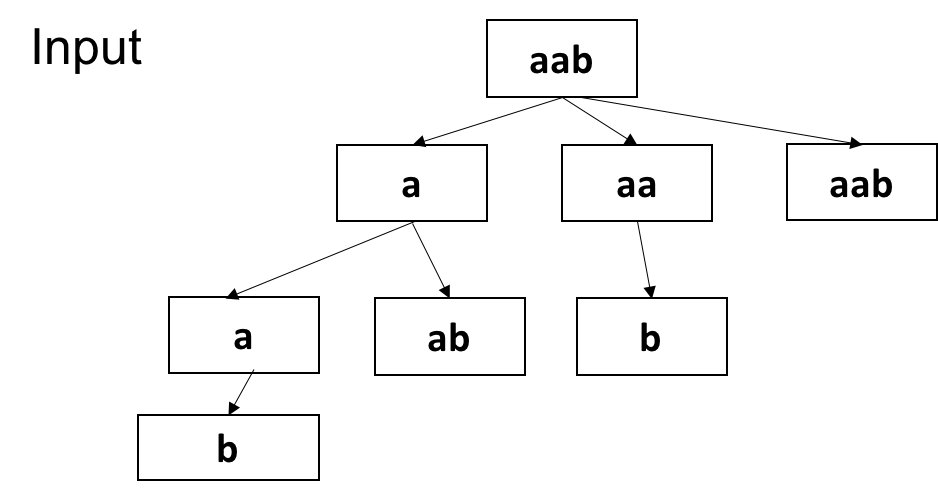
\includegraphics[width = 0.5\columnwidth]{fig/palindromPartition.png}
    \caption{State Transfer for the panlindrom splitting}
    \label{fig:my_label}
\end{figure}
\begin{lstlisting}[language = Python]
def partition(self, s):
    """
    :type s: str
    :rtype: List[List[str]]
    """
    #s="bb"
    #the whole purpose is to find pal, which means it is a DFS
    def bPal(s):
        return s==s[::-1]
    def helper(s, path, res):
        if not s: 
            res.append(path)
        for i in range(1,len(s)+1):
            if bPal(s[:i]):
                helper(s[i:],path+[s[:i]],res)
    res=[]
    helper(s,[],res)
    return res
\end{lstlisting}
Now, we use dynamic programming, for the palindrome, if substring $s(i,j)$ is panlindrome, then if $s[i-1] == s[j+1]$, then s(i-1,j+1) is palindrome too. So, for state: $f[i][j]$ denotes if $s[i:j]$ is a palindrome with $1$ or $0$; for function: $f[i-1][j+1] = f[i][j]$, if $s[i]==s[j]$, else ; for initialization: f[i][i] = True and f[i][i+1], for the loop, we start with size $3$, set the start and end index; However, for this problem, this only acts like function $bPal$, checking it in $O(1)$ time. The running time is $146$ ms.
\begin{lstlisting}[language = Python]
def partition(s):
    f = [[False for i in range(len(s))] for i in range(len(s))]

    for d in range(len(s)):
        f[d][d] = True
    for d in range(1,len(s)):
        f[d-1][d]=(s[d-1]==s[d])
    for sz in range(3,len(s)+1): #3: 3
        for i in range(len(s)-sz+1): #the start index, i=0, 0 
            j = i+sz-1 #0+3-1 = 2, 1,1
            f[i][j] = f[i+1][j-1] if s[i]==s[j] else False
    res = []  
    def helper(start, path, res):
        if start==len(s): 
            res.append(path)
        for i in range(start,len(s)):
            if f[start][i]:
                helper(i+1, path+[s[start:i+1]], res)
    helper(0, [], res)
    return res
\end{lstlisting}
This is actually the example that if we want to print out all the solutions, we need to use DFS and backtracking. It is hard to use dynamic programming and save time.
\end{enumerate}




\section{Summary}
\textbf{Steps of Solving Dynamic Programming Problems}

We read through the problems, most of them are using array or string data structures. We search for key words: ''min/max number", ''Yes/No" in ''subsequence/" type of problems. After this process, we made sure that we are going to solve this problem with dynamic programming. Then, we use the following steps to solve it:
\begin{enumerate}
    \item . 
    \item New storage( a list) $f$ to store the answer, where $f_i$ denotes the answer for the array that starts from $0$ and end with $i$. (Typically, one extra space is needed) This steps implicitly tells us the way we do divide and conquer:  we first start with dividing the sequence $S$ into $S_{(1,n)}$ and $a_0$. We reason the relation between these elements.  
    \item We construct a recurrence function using $f$ between subproblems. 
    \item We initialize the storage and we figure out where in the storage is the final answer (f[-1], max(f), min(f), f[0]). 
\end{enumerate}
Other important points from this chapter. 
\begin{enumerate}
    \item Dynamic programming is an algorithm theory, and divide and conquer $+$ memoization is a way to implement dynamic programming.
    \item Dynamic programming starts from initialization state, and deduct the result of current state from previous state till it gets to the final state when we can collect our final answer. 
    \item The reason that dynamic programming is faster because it avoids repetition computation.
    \item Dynamic programming $\approx$ divide and conquer $+$ memoization.
\end{enumerate}

The following table shows the summary of different type of dynamic programming with their four main elements. 
\begin{figure}[h]
    \centering
    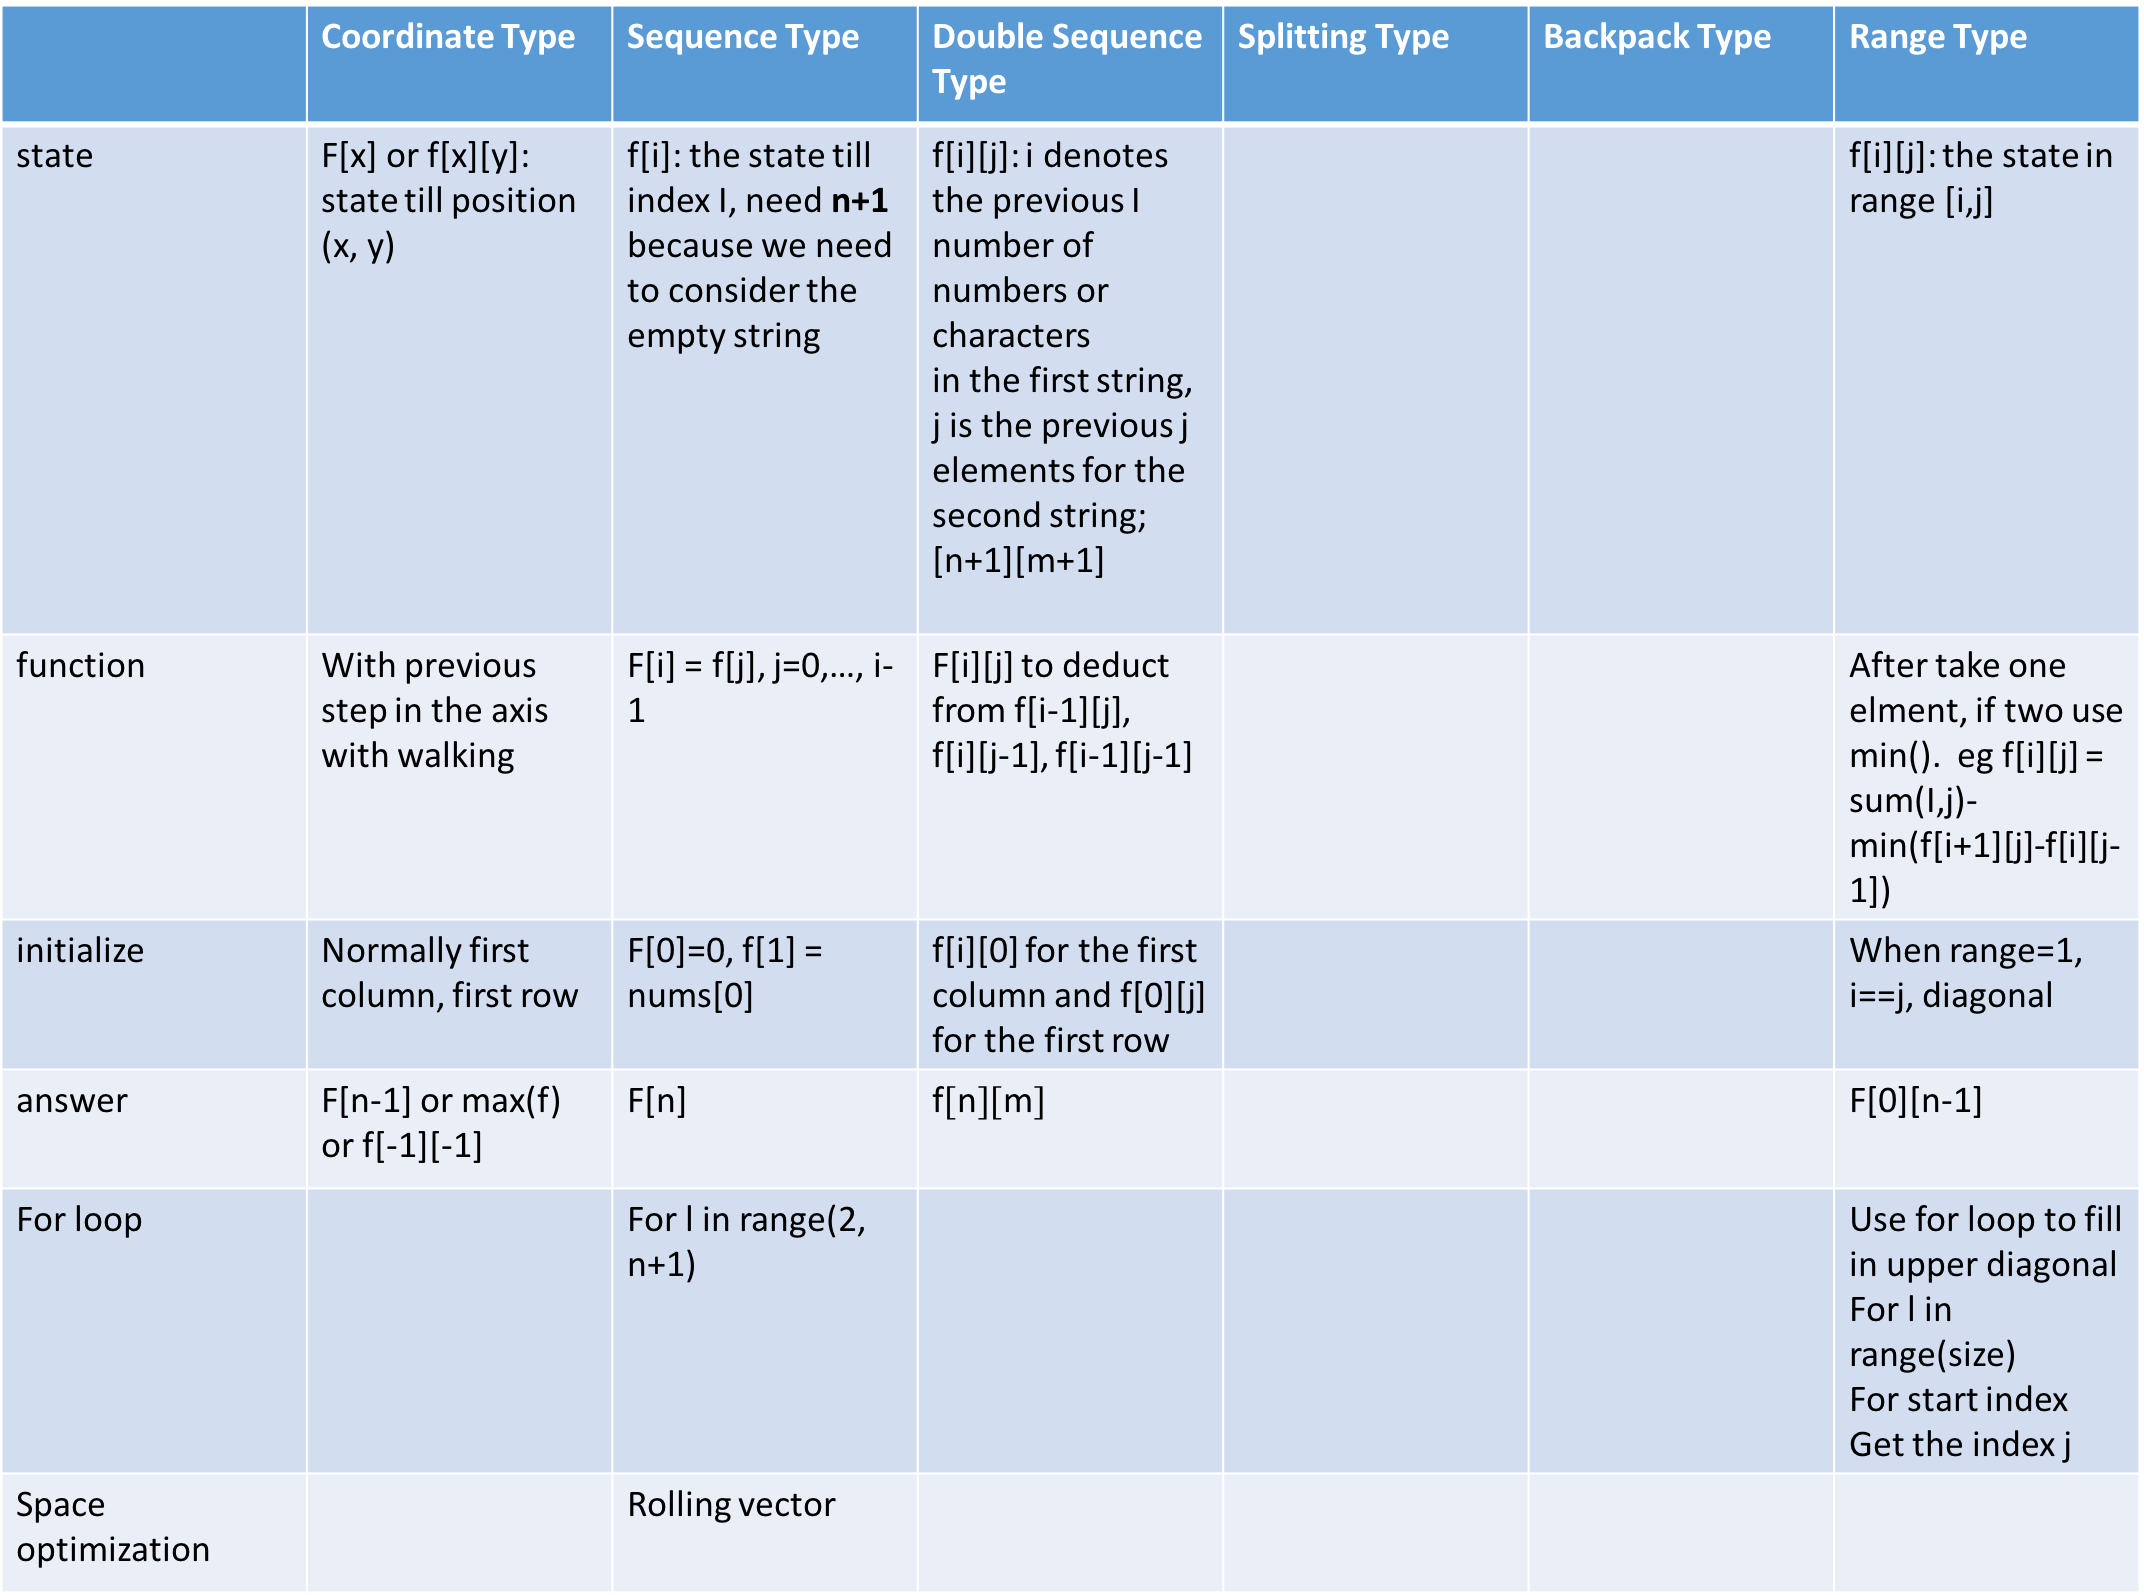
\includegraphics[width = 0.98\columnwidth]{fig/summary_dp.png}
    \caption{Summary of different type of dynamic programming problems}
    \label{fig:dp_summary}
\end{figure}

% 1.动态规划是一种算法思想,是高于算法的.而分治的记忆化搜索是实现动态规划的一种手段.
% 2.那么什么是动态规划呢?
% -就感觉上来说,动态规划的是"一层一层来",基于前一个状态推出现在的状态.
% 3.动态规划为什么会快呢?
% -因为减少了很多不必要的重复计算.
% 4.动态规划和分治的区别?
% -动态规划约等于分治+记忆化,因为有了记忆化,所以算过的直接用就行,就不用再算一遍了.
% From the brute force to recursive, to recursive with memorization, to iterative with memo, to how to save the space in memo.
\end{document}